% build with pdflatex
\documentclass[10pt]{book}										% set font size and two-sided margins (consider book tail)
\usepackage[
	paperheight=24.2cm,
	paperwidth=16.5cm,
	lmargin=26mm,
	rmargin=20mm,
	tmargin=25mm,
	bmargin=25mm,
	]{geometry}													% set S5 page size and correct margins
\usepackage[latin1]{inputenc} 									% support for swedish letters in adresses etc.
\usepackage{amsmath}  											% enables equation environments
\usepackage{bm}													% enables \bm{} command for bold math
\usepackage{graphicx} 											% enables \begin{figure} environment
\usepackage{float} 	  											% enables \begin{figure}[H] forcing of figure position using
\usepackage{setspace} 											% enables \begin{spacing} environment on front page
\usepackage{pdfpages} 											% enables direct import of .pdf files
\usepackage{qrcode}												% enables QR-codes
\usepackage{xspace}												% enables \xspace for correct spacing after "nth", see \newcommand
\usepackage{caption}											% for multiple figures side by side (LGI material data)
\usepackage{subcaption}											% for multiple figures side by side (LGI material data)
\usepackage{gensymb}											% for \degree command (degree symbol)
\usepackage{amssymb}											% for \mathbb{R} command (real numbers)
\usepackage{hyperref}											% for www.ju.se link in "ins�ttningsblad", as well as clickable toc
\usepackage{multicol}											% enables \begin{multicols} environment for multiple column itemize
\hypersetup{													% hyperlink setup
	colorlinks=true,
	linkcolor=black,
	filecolor=black,      
	urlcolor=black,
	citecolor=black,
	pdftitle={Multiscale Constitutive Modeling of Heterogeneous Engineering Materials},
	pdfpagemode=FullScreen,
}
\newcommand\tyson{\textsuperscript{th}\xspace} 					% define \tyson command for 5th, 6th, etc...
\bibliographystyle{ieeetr} 										% changes the bibliography style
\usepackage{fancyhdr} 											% custom headers and footers
\pagestyle{fancyplain} 											% all pages conform to custom headers and footers
\renewcommand{\headrulewidth}{0pt}								% remove ruler in header
\fancyhead[L]{}													% empty left header
\fancyhead[C]{}													% empty center header  
\fancyhead[R]{}													% empty right header
\fancyhead[LE]{\slshape \nouppercase{\leftmark}}								% show italic header on odd left (L) even (E) pages
\fancyfoot[C]{} 												% clear center footer
\fancyfoot[LE,RO]{\thepage} 									% alternate page numbering, left (L) odd (O), and right (R) even (E)
\newcommand\Tau{\mathcal{T}}

\begin{document}
%% !TeX root = main.tex
\begin{titlepage}
\begin{flushleft}
\includegraphics[width=0.25\paperwidth]{graphics/newSchoolLogo}
\par\end{flushleft}

\vspace*{0.1\textheight}
\noindent \begin{flushleft}
\textsf{Doctoral Thesis}
\par\end{flushleft}

\vspace{0.03\textheight}
\begin{spacing}{1.4}
\noindent \begin{flushleft}
\textsf{\textbf{\huge{Multiscale Constitutive Modeling of Heterogeneous Engineering Materials}}}
\par\end{flushleft}{\huge \par}
\end{spacing}

\vspace{0.03\textheight}
\begin{singlespace}
\noindent \begin{flushleft}
\textsf{Johan Jansson}
\par\end{flushleft}
\end{singlespace}

\vspace{0.15\textheight}

\vspace{0.05\textheight}
\begin{center}
\par\end{center}

\vfill{}
\noindent \begin{flushleft}
\textsf{J�nk�ping University}\\
\textsf{School of Engineering }\\
\textsf{Dissertation Series No. 065 \textbullet{} 2021}
\par\end{flushleft}

\end{titlepage}

\restoregeometry

\clearpage{}
												% thesis cover
%% !TeX root = main.tex
\newenvironment{bottompar}{\par\vspace*{\fill}}{}

\pagenumbering{gobble}% Remove page numbers (and reset to 1)

\begin{bottompar}  

\noindent Doctoral Thesis in Materials and Manufacturing\\

\noindent Multiscale Constitutive Modeling of Heterogeneous Engineering Materials\\

\noindent Dissertation Series No. 065\\

\noindent � 2021, Johan Jansson\\
\\
Prepared with \LaTeX{}\\

\noindent Published by\\
%Department of Materials and Manufacturing\\
School of Engineering, J�nk�ping University \\
P.O. Box 1026\\
SE-551 11 J�nk�ping, Sweden \\
Tel.: +46 36 10 10 00\\
\href{https://www.ju.se}{www.ju.se}\\
\\
Printed by STEMA AB, year 2021\\
\\
ISBN 978-91-87289-69-9

\noindent 

\end{bottompar}
													% ins�ttningsblad
\frontmatter
\chapter*{Acknowledgments}
\addcontentsline{toc}{chapter}{Acknowledgments}  				% include acknowledgments in table of contents
Acknowledge all of those who made this possible.\\

\noindent A small note. Some thesis have placed the abstract first. Order these sections as you please, but check if there is a new requirement for a specific order.\\

\vspace{20pt}

\noindent Researcher Researcherson\\
July, 2050

\cleardoublepage
\vspace*{\fill}  
\begin{center}
	\textit{Don't forget GPT is pretty useful for syntax}\\[2ex]  
	- Some guy (some add quotes here. Could also be a funky image related to the thesis.)
\end{center}
\vspace*{\fill}  
\cleardoublepage


\chapter*{Abstract}
\markboth{Abstract}{Abstract}									% sets page header on both sides to "Abstract"
\addcontentsline{toc}{chapter}{Abstract} 						% include abstract in table of contents
\noindent Summarize the area of interest and how you have contributed to it\\


\cleardoublepage

\chapter*{Sammanfattning}
\markboth{Sammanfattning}{Sammanfattning}									% sets page header on both sides to "Sammanfattning"
\addcontentsline{toc}{chapter}{Sammanfattning} 						% include Sammanfattning in table of contents
\noindent Summarize the area of interest and how you have contributed to it, but in swedish\\


\cleardoublepage

\chapter*{Thesis}
\markboth{Thesis}{Thesis}									% sets page header on both sides to "Thesis"
\addcontentsline{toc}{chapter}{Thesis}  								% include Thesis in table of contents

This thesis provides an overview and summary of the following papers:\\

\noindent
\textbf{Paper I}: \emph{Great Paper Title} by A. Authorson, C. Coauthorson.\vspace{4pt}\\
Presented at a very nice conference on some date in some location.\vspace{4pt}\\
\noindent Author contributions: Did some stuff, presented the paper at the conference.\\\vspace{5pt}

\noindent
Add your papers here.



\tableofcontents
\mainmatter
% !TeX root = main.tex
\chapter{Introduction\label{chap:1}}
\noindent \LaTeX (pronounced "LAY-tek" or "LAH-tek") is a tool for typesetting professional-looking documents. However, LaTeX's mode of operation is quite different to many other document-production applications you may have used, such as Microsoft Word or LibreOffice Writer.

\section{Why learn \LaTeX}

\noindent Various arguments can be proposed for, or against, learning to use LaTeX instead of other document-authoring applications; but, ultimately, it is a personal choice based on preferences, affinities, and documentation requirements. \\

Arguments include:
\begin{enumerate}
\item[1.] Support for typesetting extremely complex mathematics, tables and technical content for the physical sciences;
\item[2.] Facilities for footnotes, cross-referencing and management of bibliographies;
\item[3.] Ease of producing complicated, or tedious, document elements such as indexes, glossaries, table of contents, lists of figures;
\item[4.] Being highly customizable for bespoke document production due to its intrinsic programmability and extensibility through thousands of free add-ons.
\end{enumerate}

\noindent For more, check:

\href{https://www.overleaf.com/learn/latex/Learn_LaTeX_in_30_minutes#What_is_LaTeX?}{Overleaf Tutorial}




\section{Another Part of the Introduction}

\noindent \LaTeX (pronounced "LAY-tek" or "LAH-tek") is a tool for typesetting professional-looking documents. However, LaTeX's mode of operation is quite different to many other document-production applications you may have used, such as Microsoft Word or LibreOffice Writer.\\

\noindent \LaTeX (pronounced "LAY-tek" or "LAH-tek") is a tool for typesetting professional-looking documents. However, LaTeX's mode of operation is quite different to many other document-production applications you may have used, such as Microsoft Word or LibreOffice Writer.\\

\section{Problem Formulation}\label{sec:problem}
\noindent It's probably a good time to start focusing in on the issue.\\

\section{Knowledge Gaps}\label{sec:gaps}
\noindent What do we \emph{not} know:
\begin{itemize}
	\item This issue with regards to:
	\begin{itemize}
		\item Particle physics
		\item Dark matter
	\end{itemize}
	\item With emphasis on methods for determining the exact velocity of a water drop.
\end{itemize}
% !TeX root = main.tex
\markboth{}{} % remove previous chapter header from blank page before chapter start
\chapter{Research Methodology}\label{Chap:2}
A short summary of the chapter.
\section{Purpose and Aim}

\noindent Some introductory text \ref{fig:sora1}.

\begin{figure}[H]
	\centering
	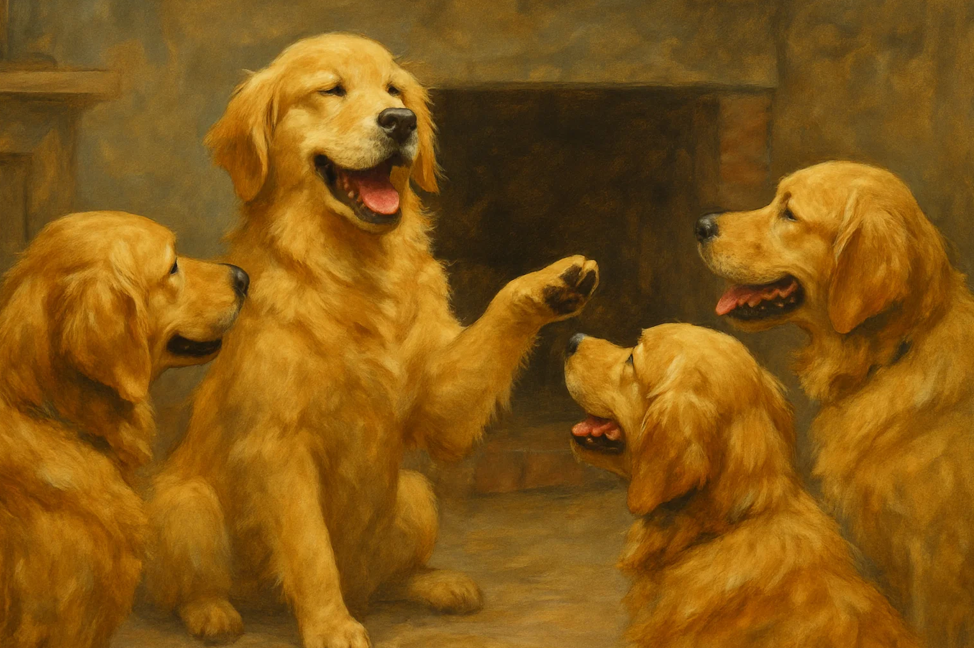
\includegraphics[scale=0.45]{graphics/Picture_1.png}
	\caption{Image generated by Sora \cite{einstein1935can}.}
	\label{fig:sora1}
\end{figure}

\noindent More introductory text.\\
 As an example, see Fig. \ref{fig:sora2}b.

\begin{figure}[H]
	\centering
	\begin{subfigure}{0.5\linewidth}
		\centering
		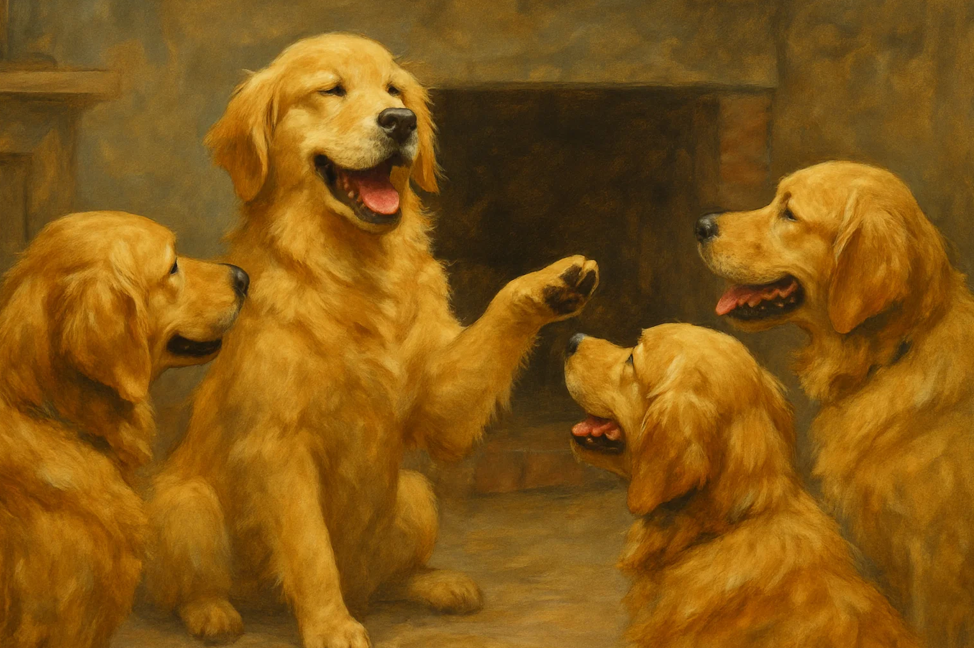
\includegraphics[scale=0.2]{graphics/Picture_1.png}		
		\caption{Dogs.}
		\vspace{-3pt}
		\label{fig:iron-mech}
	\end{subfigure}%
	\begin{subfigure}{0.5\linewidth}
		\centering
		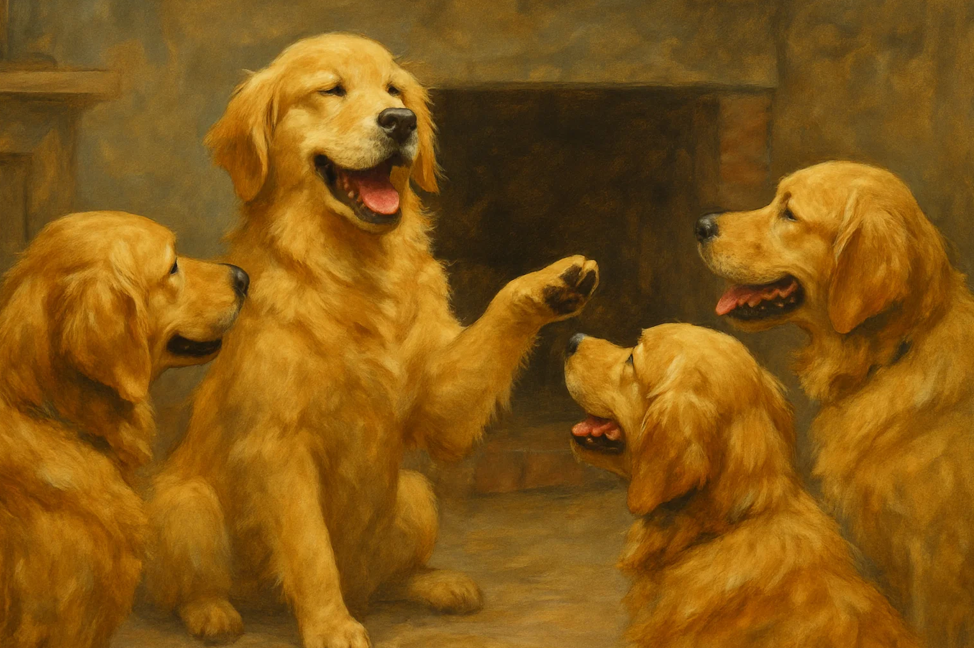
\includegraphics[scale=0.2]{graphics/Picture_1.png}		
		\caption{Same Dogs.}
		\vspace{-3pt}
		\label{fig:iron-phys}
	\end{subfigure}
	\caption{Image generated by Sora \cite{einstein1935can}.}
	\label{fig:sora2}
\end{figure}


\section{Research Design}\label{sec:2.2}

\noindent Outline your research design here.\\ 

\section{Materials and Methods}

\noindent Outline your Materials and Methods here. Don't forget to be very thorough, and, above all, clear about the limitations of your setup and methods.\\

\subsection{Of course you can also do subsections}
\subsubsection{And sub sub.} 

% !TeX root = main.tex
\chapter{Summary of Results and Discussion\label{chap:3}}
Show the main outcomes of your research in this chapter!

\noindent A way of doing equations:
(\ref{eq:max}), refer to them using these commands (\ref{eq:min}), or (\ref{eq:tat}) and perhaps (\ref{eq:tot})
\begin{align}
	\label{eq:max}\alpha & = 1\\
	\label{eq:min}\omega & = 0\\
	\label{eq:tat}\gamma & = 0\\
	\label{eq:tot}\theta & = 1.\\
\end{align}
\noindent These should look nice.

\section{Another section}
A single equation can be done as follows (\ref{eq:average})
\begin{equation}
	\rho = \frac{4}{6}\label{eq:average}
\end{equation}

% !TeX root = main.tex
\chapter{Conclusions\label{chap:4}}
Summarize your conclusions. You may add sections if needed, but its best to keep it short.




% !TeX root = main.tex
\markboth{}{} % remove previous chapter header from blank page before chapter start
\chapter{Future Work\label{chap:5}}
What could be done to improve or continue this work in the future?

% !TeX root = main.tex
\chapter{Appended Papers\label{chap:6}}

In this chapter, the appended papers are listed.

\noindent
\textbf{Paper III}: \emph{A great paper title} by A. Authorsson, C. Coauthorson and C. Coauthorson.\vspace{4pt}\\
Published in Nature, June 2050.\vspace{4pt}\\
\noindent Author contributions:\\\vspace{5pt}

\bibliography{library}											% imports the bibtex file library.bib
\addcontentsline{toc}{chapter}{Bibliography}					% adds the bibliography to the table of contents

\markboth{}{} % remove previous chapter header from blank page before chapter start
\chapter*{Paper I}
\hrule
\vspace{12pt}
\textbf{Title of the Paper} \vspace{6pt}\\
\noindent \emph{A. Authorsson, C. CoAuthorsson}  \vspace{6pt}\\

\noindent Presented at a very fancy conference on some date in some location.
\markboth{}{}													% clear page header on both sides
\addcontentsline{toc}{chapter}{Paper I} 						% include paper I in table of contents
\cleardoublepage{} 												% makes the next page a right-hand (odd-numbered) page, producing a blank page if necessary.
\markboth{Paper I}{Paper I}										% sets page header on both sides to "Paper I"

%Comment the next lines out if you want to add PDF's to your thesis. Otherwise send them separately to the printing company.

%\includepdf[pages=-,offset=5mm -3mm,noautoscale = true,scale=.77,pagecommand={\pagestyle{fancyplain}}]{papers/name of the document}
%\markboth{}{}													% clear page header on both sides


\end{document}